\chapter{Uvod}\label{ch:uvod}

Aplikacije koje su namenjene za globalno tržište treba pripremiti 
tako da korisnici koji pripadaju različitim govornim područjima i 
geografskim regionima razumeju sadržaj. Postupak dizajniranja aplikacije 
tako da podrži različite jezike se naziva internacionalizacija, a osobina 
aplikacije koja podržava više jezika se naziva višejezičnost. 

Proces prilagođavanja softvera za različite jezike može biti kompleksan. 
Veliku pomoć u tom procesu danas pružaju različita rešenja. Odabir rešenja 
uglavnom zavisi od odabira programskog jezika u kom će softver biti 
razvijan, kao i od korišćenja programskog okvira.

Sa druge strane, ne može se očekivati da programer zna sve jezike za koje je 
softver namenjen. To znači da se u proces internacionalizacije uključuju i 
prevodioci koji poznaju jezik korisnika. Oni implicitno 
postaju osobe koje razvijaju softver.

Pomenuta rešenja za olakšavanje internacionalizacije uglavnom su fokusirana
samo na tehničke probleme, odnosno probleme programera. Prevodi se čuvaju u
fajlovima i obično predstavljaju serijalizovanu strukturu mape, odnosno parove
"ključ -- vrednost". Takvi fajlovi su neretko teški za korišćenje od strane
netehnikičih lica, a prevodioci često nisu tehnička lica. Kako bi što bolje 
obavljali svoj posao, prevodiocima je potrebna neka vrsta alata koja im deluje
poznato, nešto na šta su navikli, odnosno nešto što koriste svaki dan. 
Prevodioce ne zanima koje rešenje su programeri izabrali, niti koji format 
serijalizacije se koristi. Njima je potreban familijaran interfejs za ažuriranje
tih fajlova.

Razvojem računarstva u oblaku, ljudi su navikli da im se sve nalazi u oblaku, 
odnosno da im je sve uvek dostupno, na svakom mestu i u bilo koje vreme. 
Paralelno sa razvojem softvera u oblaku, popularnost stiču arhitekture zasnovane
na mikroservisima ali i razvoj aplikacija u kontejnerima. Za kontrolisanje 
velikog broja kontejnera se sve više korsti alat \textit{Kubernetes}. Pored toga, 
tendencija je da se hardver, odnosno infrastruktura, više ne održava u okviru
organizacije, već da se on iznajmljuje od dobavljača računarstva u oblaku 
(eng. \textit{Cloud Computing Provider}). Ovakvim pristupom se omogućava lako 
prenošenje aplikacije sa jednog okruženja na drugo. Razvoj takvog softvera nosi
sa sobom dodatne izazove. 

U ovom radu biće opisan razvoj softvera u oblaku. Fokus će biti stavljen na 
arhitekturu mikroservisa, korišćenje alata \textit{Kubernetes} i proces pravljenja 
višejezične aplikacije. Za razvoj klijentskog, ali i serverskog dela 
kôda, koristiće se programski jezik \textit{JavaScript}. U svrhu ilustracije i
boljeg razumevanja biće razvijena aplikacija za upravljanje prevodima. 
Implementirano rešenje je nazvano \textit{Interpres}. Aplikacija je 
višejezična, odnosno može prikazati korisnički interfejs u više 
jezika. Za potrebe uređivanja prevoda je korišćen upravo \textit{Interpres}.
Izvorni kod je otvoren i može se naći na \url{https://github.com/enco164/interpres}.

\section{Problem prevođenja}\label{ch:analiza}

Analizom postojećih alata za upravljanje prevodima mogu se uočiti prednosti i mane tih alata. 
Zadatak analize postojećih sistema je upoznavanje sa problematikom kako bi se izbegle greške
koje su ti sistemi napravili, ali i prikupljanje dobrih ideja i funkcionalnosti koje pružaju ti sistemi.


\subsection{Postojeća okruženja}\label{sec:analiza-postojeca_okruzenja}

Na tržištu postoji dosta rešenja koji se bave upravljanjem prevodima. Jedno od takvih rešenja je 
\textit{BabelEdit}~\cite{BabelEdit}, editor prevoda za veb aplikacije. Program se instalira na klijentskom računaru.
Program podržava pravljenje projekta u koji se kasnije uvoze fajlovi sa prevodima. Kada korisnik završi 
sa prevođenjem, može da izveze prevode iz projekata u razne formate. Ovaj alat ne nudi mogućnost kolaboracije,
a fajlovi se nalaze na lokalnom računaru, i kao takav je pogodan jedino za manje projekte. Ovaj alat ima 
probni period od nekoliko dana, a kasnije se mora platiti.

Drugo popularno rešenje je \textit{Localazy}~\cite{Localazy}, platforma koja podržava više od 50 radnih okvira, 
formata fajlova. Platforma se nalazi u oblaku i pristupa joj se preko veb pregledača. Na platformi se može 
napraviti novi projekat u okviru kojeg se mogu uvesti fajlovi sa prevodima za izabrani jezik. Istom projektu 
može pristupiti više prevodilaca i uređivati prevode. Kada se izabere fajl za prevod, sa leve strane se može 
videti ključ za nisku koju treba prevesti, a pored njega i sam prevod. Prevodi su kasnije dostupni preko 
mreže za dostavu sadržaja (eng. \textit{Content Delivery Network, CDN}). \textit{Localazy} omogućava besplatno korišćenje za 
projekte koji imaju najviše 200 ključeva, što odlikuje manje projekte.

Navedeni alati poseduju i integraciju sa sistemima za mašinsko prevođenje, što u mnogome olakšava posao 
prevodiocima. Svakako, na kraju je potrebna provera od strane čoveka kako bi sadržaj bio u većoj meri prilagođen. 


\subsection{Moguća unapređenja}\label{sec:analiza-moguca_unapredjenja}

Oba analizirana alata pružaju nekakav oblik obaveštenja da je prevodilac završio sa poslom. U slučaju alata \textit{BabelEdit}
potrebno je da prevodilac izveze prevode i kasnije izvezene fajlove da pošalje programeru. Kod \textit{Localazy} 
je proces malo bolji jer prevodilac ne treba da šalje nikakve fajlove, već samo da obavesti programera, 
koji će ih kasnije preuzeti sa \textit{CDN}.

Ovde se može primetiti da je moguće automatizovati proces predaje prevoda. Potrebno je samo da klikom dugmeta
prevodilac obavesti sistem da je završio svoj posao. Ta akcija bi trebalo da pokrene izgradnju nove verzije aplikacije.
\chapter{Arhitektura i dizajn sistema}\label{ch:arhitektura}

Funkcionalni zahtev da aplikacija bude u oblaku, opisan u poglavlju 
\ref{sec:funkcionalni_zahtevi-aplikacija_u_oblaku}, nameće grubu sliku kako arhitektura sistema 
treba da izgleda. Aplikacije na vebu su dominantno bazirane po modelu klijent--server arhitekture. 
Server u takvoj arhitekturi obezbeđuje uslugu klijentima koji je zahtevaju. Klijent--server 
arhitektura je višenamenska i modularna, a sa ciljem unapređenja upotrebljivosti, interoperabilnosti, 
fleksibilnosti i skalabilnosti. 

Veb aplikacije su nezavisne od platforme jer zahtevaju samo veb pregledač, dok se kod standardne 
klijent--server arhitekture klijent mora instalirati na platformi korisnika. Pored toga, 
kod veb aplikacija je protokol komunikacije definisan, koristi se \textit{HTTP}, dok se kod klijent--server
arhitekture protokol može izabrati po potrebi.

Komponente klijent -- server arhitekture, prilagođene za veb, se mogu grupisati u tri kategorije: 
server, klijent i mreža. Uloga servera je da upravlja zajedničkim resursima, bazom podataka, da 
izvršava poslovnu logiku, kao i da kontroliše pristup i bezbednost podataka. Posao klijenta je da 
upravlja korisničkim interfejsom. Računarska mreža omogućava komunikaciju između klijenta i servera, 
a komunikacija mora pratiti određene standarde.

\section{Arhitektura teških klijenata}\label{sec:arhitektura-spa}

Odlika arhitekture teških klijenata je da server šalje klijentu podatke i meta podatke, i prepušta 
mu da samostalno pripremi prezentaciju.~\cite{PVEB} Ovakvom podelom odgovornosti se smanjuje opterećenje 
servera, jer više ne mora da priprema prezentaciju. Arhitektura teških klijenata podrazumeva intenzivno 
korišćenje \textit{JavaScript}-a.

Ekstremni oblik ove arhitekture je arhitektura jedne stranice (eng. \textit{SPA - Single Page Application}).
Arhitektura jedne stranice propisuje da se čitava aplikacija učitava kroz jednu stranicu. Primenom 
ovih pravila se dobija potpuno odvojen klijent od servera. Klijent u ovom slučaju komunicira 
sa serverom u pozadini radi preuzimanja podataka i izvođenja transakcija. S obzirom da prezentacija
priprema na korisničkoj strani, korisnički interfejs ima bolji odziv, jer se ne prenosi kroz mrežu.

\section{Mikroservisi}\label{sec:arhitektura-mikroservisi}

Tradicionalan način razvijanja poslovnih aplikacija predstavlja razvoj takozvane monolitne arhitekture. 
Jedan monolit bi sadržao svu poslovnu logiku koju izvršava aplikacija. Kako aplikacija raste vremenom, 
tako raste i sam monolit, koji se sve teže održava. Problemi koji nastaju kod velikog monolita nisu 
samo problemi održavanja, već je i skaliranje upitno. Njih karakteriše spor razvojni ciklus i ažuriraju se relativno retko.

Danas se ovako veliki monoliti raščlanjuju na manje, nezavisne komponente koje se nazivaju mikroservisima. 
Džejms Luis i Martin Fauler kažu da se izraz "Mikroservisna arhitektura" sve češće pojavlje poslednjih 
par godina kako bi opisao određeni način projektovanja softverskih aplikacija kao paketa usluga koji se 
mogu odvojeno isporučiti. Iako ne postoji precizna definicija ovog arhitektonskog stila, postoje određene 
zajedničke karakteristike u organizaciji oko poslovne logike, automatskog isporučivanja i decentralizovane 
kontrole podataka.~\cite{martinfowler_microservices} 

Mikroservisi predstavljaju aplikaciju koja je struktuirana kao kolekcija slabo vezanih servisa. Glavna 
ideja iza mikroservisne arhitekture je da se aplikacije lakše razvijaju i održavaju ako su podeljene 
na manje delove koji rade nesmetano zajedno.

Servisi se mogu posmatrati kao komponente sistema. Martin Fauler definiše komponente kao jedinice 
softvera koje se mogu nezavisno zameniti i unaprediti.~\cite{martinfowler_software_component}.

Biblioteke su komponente koje su povezane u program i pozivaju se pomoću funkcija koje se nalaze u 
memoriji, dok su servisi komponente koje su van procesa i koje komuniciraju preko mreže.
Servisi, naravno, mogu da koriste biblioteke. Glavni benefit ovakvog korišćenja servisa je da se mogu 
nezavisno isporučiti, što nije slučaj ako imamo jednu aplikaciju koja je sastavljena od skupa biblioteka.
Sa druge strane, daljinski pozivi preko mreže su skuplji, odnosno sporiji. 
Druga loša strana je da se logika teže prebacuje iz jednog servisa u drugi, odnosno refaktorisanje je 
otežano u tom smislu.

Da bi se monoliti lakše razvijali, programeri se uglavnom podele po tehnologiji, na primer u tim za 
bazu podataka, tim za poslovnu logiku i tim za korisnički interfejs. U arhitekturi mikroservisa je malo 
drugačije. Timovi se organizuju oko jednog servisa i sastavljeni su od progamera različitih tehnologija.
To znači da su timovi nezavisni, kao i što su i sami servisi nezavisni, i organizovani su sa fokusom na 
poslovnu logiku, a ne na tehnologiju.

Jedna zgodna posledica deljenja monolita na servise je da servisi ne moraju da budu razvijeni u istim 
tehnologijama. Tako na primer, jedan servis može biti izgrađen u programskom jeziku \textit{C++} a drugi u 
\textit{NodeJS}, dokle god mogu da komuniciraju jedan sa drugim. Nekada je pogodnije koristiti drugi programski 
jezik jer je u njemu lakše rešiti problem.

Monolitne aplikacije preferiraju da imaju jednu bazu podataka za čuvanje podataka. Sa druge strane, kod 
mikroservisnih aplikacija se odluka o bazi podataka prepušta samom servisu. Neke probleme koje servis 
rešava je pogodnije rešiti relacionom bazom podataka, dok je za neki drugi servis možda pogodnija grafovska baza.
Iako i monolitne aplikacije mogu da koriste više tipova baza podataka, ova osobina je češća kod 
mikroservisa. Decentralizovana odgovornost za čuvanje podataka ima i svoje implikacije na ažuriranje 
podataka. Ovaj problem se može rešiti korišćenjem transakcija. Korišćenjem transakcija rešava se problem 
konzistentnosti, ali se smanjuje dostupnost. Zato, česta je odluka da se konzistentnost zameni 
odloženom konzistentnošću, u onim slučajevima gde je ona moguća. 

Kada se govori o mikroservisima često se, sa razlogom, postavlja pitanje postoji li razlika između arhitekture
mikroservisa i servisno orijentisane arhitekture (eng. \textit{Service Oriented Architecture}, \textit{SOA}). 
Glavne karakteristike arhitekture mikroservisa su umnogome slične \textit{SOA}. Problem je taj što \textit{SOA} 
može da predstavlja mnogo različitih stvari. Preveliki fokus na kanal komunikacije 
(eng. \textit{Enterprise Service Bus}, \textit{ESB}) koji se koristi za integraciju monolitnih aplikacija, 
predstavlja jedan od tih problema. Može se reći da je arhitektura mikroservisa nastala iz stečenog iskustva tokom 
razvijanja \textit{SOA}, odnosno da predstavlja sledeći iterativni korak u razvoju ove arhitekture. 
Preuzeti su raznorazni dobri obrasci iz \textit{SOA}. Sa druge strane, delovi koji su bili previše kompleksni 
zamenjeni su jednostavnijim. Primer je \textit{ESB} koji je zamenjen jednostavnijim veb protokolima. 

Ljudi koji zagovaraju arhitekturu mikroservisa su iz navedenih razloga krenuli da odbacuju naziv \textit{SOA}, 
dok drugi smatraju da su mikroservisi samo još jedan oblik \textit{SOA}. Baš zato što \textit{SOA} 
može da predstavlja toliko različitih stvari, dragoceno je imati izraz koji preciznije opisuje arhitekturu 
zvanu mikroservisi.~\cite{martinfowler_microservices}

\section{REST}\label{sec:arhitektura-rest}

Interoperabilnost je sposobnost da različiti sistemi rade zajedno. Da bi se ovo postiglo potrebni su 
standardi koje će sistemi poštovati. Kako u klijent -- server arhitekturi imamo dva različita sistema 
(klijent i server), oni moraju poštovati određene standarde za komunikaciju. Jedan od takvih standarda za 
komunikaciju je i \textit{REST} (eng. \textit{Representational State Transfer}). \textit{REST} je stil 
softverske arhitekture koji definiše skup pravila koja treba da se poštuju tokom pravljenja mrežnih 
aplikacija. Prvi put je predstavljen u doktorskoj disertaciji Roja Fildinga~\cite{REST_Roy}. Po \textit{REST}-u, 
fokus se prebacuje sa procedura na resurse (objekte). Za aplikaciju kažemo da je \textit{RESTful} ako poštuje pravila REST-a.


\textit{REST} definiše šest pravila koja moraju da se ispoštuju~\cite{REST_API}:

\begin{itemize}

	\item \textbf{Klijent -- server}: Razdvajanjem korisničkog interfejsa od servera briga o podacima 
	ostaje na serveru. Klijenti postaju lakši za portabilnost među različitim sistemima, a server se može
    lakše skalirati.
	
    \item \textbf{Sistem bez stanja (eng. \textit{Stateless})}: Svaki zahtev sa klijenta ka serveru mora da sadrži 
	sve potrebne informacije da bi zahtev bio opslužen. Klijent se ne sme oslanjati na stanje servera. 
    Zapravo, stanje na serveru se zabranjuje. Iz tog razloga stanje sesije se u potpunosti čuva na klijentu.
	
    \item \textbf{Keširanje}: Server u svom odgovoru sa nekim podacima mora eksplicitno da navede da li 
    podaci mogu da se keširaju, ili ne. Ako server odgovori da su podaci kešabilni, klijent ih može 
    koristiti kasnije ako je zahtev za podacima isti. Server može napomenuti i vreme isteka keša.
    
    \item \textbf{Uniforman interfejs}: Uniforman interfejs definiše interfejs između klijenta i servera.
    On pojednostavljuje i razdvaja arhitekturu, što omogućava da se svaki deo razvija samostalno. 
    Četiri vodeća principa uniformnog interfejsa su:

    \begin{enumerate}
        \item \textbf{Zasnovanost na resursima}: Individualni resursi se mogu identifikovati u 
        zahtevima koristeći \textit{URI} kao identifikator resursa. Resursi kao takvi su konceptualno odvojeni 
        od reprezentacije koja se vraća klijentima. Na primer, server ne šalje svoju bazu podataka, 
        već radije, šalje \textit{HTML}, \textit{XML} ili \textit{JSON} koji predstavljaju traženi zapis iz baze podataka.

        \item \textbf{Upravljanje resursima kroz reprezentaciju}: Kada klijent sadrži reprezentaciju resursa,
        uključujući meta podatke u prilogu, onda ima dovoljno podataka da izmeni ili obriše resurse 
        sa servera, pod uslovom da ima ovlašćenje da to uradi.

        \item \textbf{Samoopisne poruke}: Svaka poruka sadrži dovoljno informacija da opiše na koji 
        način treba da bude obrađena. Na primer \textit{Internet media type} (nekada poznat pod nazivom \textit{MIME}) 
        može sadržati informaciju o tome koji parser treba da se pozove. Odgovori eksplicitno 
        označavaju da li imaju sposobnost keširanja.

        \item \textbf{Hipermedija kao pokretač aplikacije (\textit{HATEOAS})}:
        Klijenti treba da znaju što je manje moguće o tome kako da komuniciraju sa serverom. Komunikacija treba da bude
        što je više moguće generička. Server svoje stanje isporučuje klijentu u vidu hiperteksta, koji unutar sebe 
        sadrži hiperlinkove. To se tehnički naziva hipermedija (hiperlinkovi unutar hiperteksta). 
        \textit{HATEOAS} (eng. Hypermedia as the Engine of Application State) 
        znači da, tamo gde je potrebno, veze su sadržane unutar vraćenog odgovora. 
        Tako se isporučuje URI za preuzimanje samog objekta ili srodnih 
        objekata. Uniformni interfejs koji svaki \textit{REST} servis mora pružiti je fundamentalna 
        osnova za njegov dizajn.
        
        
    \end{enumerate}
    
	\item \textbf{Slojevit sistem}: \textit{REST} omogućava korišćenje slojevitih sistema, gde klijent ne zna 
    eksplicitno da li komunicira sa krajnjim serverom ili sa posrednikom. Ovako se može povećati 
    skalabilnost uvođenjem balansera opterećenja ili uvođenjem keširanja na strani servera. 
	
	\item \textbf{Kod na zahtev (opciono)}: Serveri mogu obogatiti klijentsku stranu slanjem koda koji će biti izvršen na 
	klijentskoj strani. Ovo može uprostiti klijente jer se smanjuje broj funkcija koje je potrebno da 
    klijent ima. Primer na vebu bi bio slanje \textit{JavaScript} koda. 

\end{itemize}



\section{Tehnologije korišćene u radu}\label{ch:tehnologije}

U ovom poglavlju će biti opisane tehnologije korišćene za razvoj rešenja, a prateći ranije opisanu arhitekturu.

\subsection{React}\label{sec:react}
\textit{React} je \textit{JavaScript} biblioteka za građenje korisničkog interfejsa. Koristi se za pravljenje modernih 
reaktivnih korisničkih interfejsa koji se mogu izgraditi uz pomoć izolovanih delova koda. Ti delovi koda nazivaju 
se komponente. Korišćenjem komponenti omogućeno je deljenje aplikacije na nezavisne delove koji se prilikom razvoja 
mogu iznova koristiti~\cite{react}.

Svaka komponenta sastoji se iz metode za renderovanje i sadrži podatke o tome šta je sve potrebno da se prikaže 
krajnjem korisniku. Komponente mogu biti klasne ili funkcijske. Funkcijske komponente (eng. \textit{function components}) kao ulazni parametar primaju svojstva
i vraćaju \textit{JSX} element. Sa druge strane, klasne komponente su definisane kao \textit{ES6} 
klase i renderuju \textit{React} elemente koristeći \texttt{render()} metodu. 

Kako bi komunicirale međusobno sa ostalim delovima aplikacije, komponente moraju imati svoje stanje (engl. \textit{state}) 
i svojstva (eng. \textit{properties - props}). Svojstva i stanje predstavljaju čist \textit{JavaScript} objekat. Izmena bilo kojeg 
od ova dva objekta okida ponovno renderovanje komponente. 

Svojstva čine \textit{React} komponente fleksibilnim i pogodnim za 
ponovno korišćenje. Prosleđivanjem različitih svojstava, komponente se mogu ponašati i izgledati drugačije. Svojstva komponente 
služe isključivo za prikaz i unutar same komponente ih ne bi trebalo menjati. Protok informacija mora biti jednosmeran od višeg 
nivoa komponente ka nižem. Stoga je komponenta sa višeg nivoa zadužena za prosleđivanje skupa svojstava.

Stanje komponente se koristi za "pamćenje" podataka unutar same komponente. Možemo reći da je stanje privatno, jer se stanju 
komponente ne može pristupiti iz roditeljske komponente. Može se promeniti na osnovu korisnikove interakcije ili neke druge 
akcije unutar aplikacije. Za razliku od svojstava, stanjem se može upravljati unutar same komponente.

\textit{React} kuke (eng. \textit{hooks}) služe za korišćenje stanja u funkcijskim komponentama. U teoriji, kuke su funkcije
koje se "kače" za stanja i životne cikluse unutar funkcijske komponente. Da bi se koristile \textit{React} kuke, moraju se 
poštovati dva pravila:
\begin{itemize}
    \item Pozivanje kuka se mora vršiti sa najvišeg nivoa. To znači da se one ne smeju pozivati unutar petlji, 
    postavljenih uslova ili ugnježdenih funkcija.
    \item Pozivanje kuka se ne može vršiti iz običnih \textit{JavaScript} funkcija, već samo iz funkcija \textit{React} komponente.
\end{itemize}

Stanje svake komponente je potpuno nezavisno. Korišćenjem kuka, postiže se to da se logika sa stanjem može ponovo koristiti 
(ali ne i samo stanje). U stvari, svakim pozivom kuke dobijamo potpuno izolovano stanje, pa se stoga jedna kuka može koristiti 
više puta unutar jedne komponente. Pored toga, kuke omogućavaju pravljenje kompozicije. Unutar jedne kuke je moguće zakačiti 
drugu kuku i tako napraviti kompoziciju. 

Pre uvođenja kuka, u \textit{React}-u se koristio obrazac zvan "komponente višeg reda" (eng. \textit{Higher-Order Components}). 
Konkretno, komponenta višeg reda je funkcija koja za argument prihvata komponentu i vraća novu komponentu. Kako su i ulaz i 
izlaz istog tipa (\textit{React} komponenta), lako se može zaključiti da se komponente višeg reda mogu komponovati, a logika i 
stanje koje one dodaju se mogu iskoristiti na više različitih mesta. Iako je i dalje moguće koristiti ovaj obrazac, jer je 
nezavisan od toga da li je komponenta napisana kao klasa ili kako funkcija, preporučuje se koršćenje kuka, kad god je moguće. 
Naime, kuke imaju dve glavne osobine koje imaju i komponente višeg reda: ponovno korišćenje i kompoziciju. Glavna prednost kuka 
u odnosu na komponente višeg reda je to što su zavisnosti eksplicitne kod kuka. Sa druge strane, kuke se mogu koristiti samo u 
funkcijskim komponentama pa je upotreba komponenti višeg reda opširnija.

Glavna prednost \textit{React} kuka je enkapsulacija. Odgovornost za prikazivanje korisničkog interfejsa ostaje na samoj 
komponenti, a logika prikaza za tu komponentu se prebacuje u kuku koja se vezuje za tu komponentu. Na taj način se štiti 
od neželjenog pristupa unutrašnjim podacima od strane komponente i sakriva se kompleksnost. Uz sve navedeno, 
testiranje postaje lakše jer se odvojeno mogu testirati prikaz korisničkog interfejsa i logika prikaza. Praktično,
testovi za kuke, odnosno logike prikaza, postaju testovi jedinice koda (eng. \textit{Unit Test}) a testovi prikaza
korisničkog interfejsa postaju integracioni testovi (eng. \textit{Integration Test}).

Prilikom razvoja aplikacije susrećemo se sa izazovima kao što je pravljenje konzistentnih komponenti koje izgledaju i funkcionišu 
na isti način, ne samo unutar jedne aplikacije već i na mnogim drugim aplikacijama koje se razvijaju. Ispis identičnih stilova 
komponenata iznova i izmena promenljivih vrednosti na više mesta u aplikaciji utiče na vreme razvoja aplikacije.

Umesto da se stilovi koriste globalno, teži se ka tome da se postave standardizovane komponente sa ugrađenim funkcionalnostima i 
stilovima kako bi se one mogle koristiti iznova i podešavati jednostavno u zavisnosti od slučaja u kojem se koriste.
Jedna od popularnijih biblioteka za stilizovanje \textit{React} komponenata je \textit{Material UI}. Ona predstavlja 
implementaciju \textit{Google}-ovog \textit{Material Design}-a. Uz pomoć ove biblioteke komponente se mogu koristiti zasebno, 
koristeći samo one stilove koji treba da budu prikazani.

\textit{Material UI} biblioteka koristi \textit{CSS} u \textit{JS} (eng. \textit{CSS-in-JS}). Korišćenjem globalnih \textit{CSS} 
fajlova, a zbog kaskadne prirode \textit{CSS}-a (\textit{Cascading Style Sheets}), stilovi se mogu učitati u bilo kom redosledu 
i pregaziti neki drugi stil. Pisanjem \textit{CSS} u \textit{JavaScript}-u rešava problem zavisnosti jer se mogu koristiti 
\textit{JavaScript} moduli. Na taj način se komponente mogu pokretati nezavisno, bez oslanjanja na eksterne \textit{CSS} fajlove. 
Kako danas većina alata za izgradnju projekta podržava pronalaženje i brisanje koda koji se ne koristi, a samim tim i smanjuju 
veličinu izgrađenog projekta, ova tehnika se može primeniti i na \textit{CSS} u \textit{JS}. Stilovi su opisani preko 
\textit{JavaScript} objekata i kao takvi mogu da pristupe stanju komponente što povećava fleksibilnost pisanja samih stilova.


\subsection{NestJS}\label{sec:nestjs}
Razvoj aplikacije na \textit{Node.js} platformi vremenom može postati kompleksan. Što se više svojstava 
dodaje u aplikaciju, to baza koda postaje sve veća.

\textit{NestJS} je radni okvir za građenje efikasne skalabilne \textit{Node.js} aplikacije na serveru. 
Pruža serverskom delu aplikacije modularnu strukturu za organizaciju koda u odvojene module i služi 
za eliminisanje neorganizovane baze kodova.

Korišćenjem \textit{NestJS} programerima se pruža mogućnost da koriste sve benefite JavaScript-a i uz
to pišu kod za klijentski i serverski deo aplikacije u istom programskom jeziku. Sadrži komponente 
funkcionalnog, objektno orijentisanog i funkcionalno reaktivnog programiranja.

Inspirisan \textit{Angular}-om, \textit{NestJS} je napisan u programskom jeziku \textit{TypeScript} 
i koristi \textit{Express.js}, koji ga čini kompatibilnim sa većinom \textit{Express} posredničnih 
(eng. \textit{middleware}) softvera. Za razvoj podržava JavaScript i TypeScript, kao i PostgreSQL, 
MongoDB i MySQL baze podataka.

Osnovne gradivne komponente NestJS aplikacije su kontroleri, provajderi i moduli.

Kao i kod većine radnih okvira, kontroleri u \textit{NestJS} su odgovorini za opsluživanje zahteva koji dolaze
sa klijentske strane. \textit{NestJS} je struktuiran tako da je
mehanizam za usmeravanje, prikazan na slici \ref{fig:kontroler}, sposoban da kontroliše koji kontroler 
će biti zadužen za određeni zahtev.
Kako bi se napravio osnovni kontroler, koriste se klase i dekoratori. Dekoratori pridružuju meta
podatke klasama i omogućavaju \textit{Nest}-u da napravi mapu za rutiranje. Za definisanje HTTP 
metoda za rute, koriste se dekoratori \texttt{@Get()}, \texttt{@Put()}, \texttt{@Post()} i \texttt{@Delete()}~\cite{nest}.

\begin{figure}[h]
    \centering
    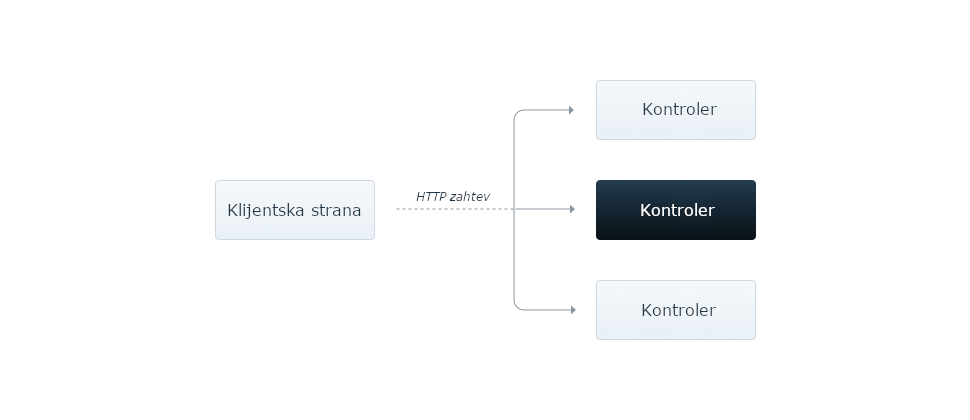
\includegraphics[width=1\textwidth]{kontroler}
    \caption{Usmeravanje zahteva}
    \label{fig:kontroler}
\end{figure}
  
\textit{Nest} provajderi se mogu umetnuti u kontrolere ili u druge provajdere. Nazivaju se i servisi, 
i dizajnirani su da apstrahuju bilo koji oblik složenosti i logike.
Servisni provajder u \textit{Nest} je klasa sa specijalnim dekoratorm \texttt{@Injectable()}. 

Moduli omogućavaju grupisanje povezanih fajlova. To su TypeScript fajlovi dekorisani sa 
\texttt{@Module} dekoratorom, koji pruža meta podatke koje \textit{Nest} koristi za organizaciju 
strukture aplikacije. Svaka \textit{Nest} aplikacija mora imati bar jedan modul -- osnovni modul. 
Preporučuje se da se velike aplikacije rastave na više modula kako bi se lakše kontrolisala 
struktura aplikacije.

Tri osnovna koncepta NestJS su:
\begin{itemize}
\item \textbf{DTO}: Objekat za prenos podataka (eng. \textit{Data Transfer Object}) je objekat 
koji definiše kako će se podaci poslati preko mreže;
\item \textbf{Interfejsi} : \textit{TypeScript} interfejsi se koriste za proveru tipa i 
definisanje tipova podataka koji se mogu proslediti kontroleru ili \textit{NestJS} servisu i
\item \textbf{Umetanje zavisnosti} (eng. \textit{Dependency Injection}) je obrazac projektovanja 
koji se koristi za povećanje efikasnosti i modularnosti aplikaicje. Održava kod čistim i 
lakšim za korišćenje. U \textit{NestJS} se koristi za pravljenje uvezanih komponenata~\cite{nest_getting_started}.
\end{itemize}

\subsection{GitHub aplikacija}\label{sec:github_app}
Aplikacije na \textit{GitHub}-u mogu automatizovati i poboljšati tok razvoja. \textit{GitHub} 
aplikacije se preporučuju za integrisanje sa \textit{GitHub}-om jer nude granularnije permisije 
za pristup podacima. 

\textit{GitHub} aplikacije se mogu instalirati direktno na organizacione i korisničke naloge i 
odobriti pristup specifičnim repozitorijima. Može ih instalirati vlasnik naloga organizacije 
ili korisnik sa administratorskim dozvolama. Kako bi ih promovisao, \textit{GitHub} je napravio
stranicu koja predstavlja prodavnicu aplikacija i preko ove prodavnice je moguće instalirati 
aplikacije i dodatno obogatiti repozitorijume.

\textit{GitHub} aplikacije se ponašaju kao dodatni korisnici na repozitorijumu. Za svaku 
aplikaciju se vezuje jedan identitet koji joj odgovara. Registrovanjem aplikacije programer 
dobija pristupne ključeve. Uz pomoć ovih ključeva i \textit{GitHub}-ovom bibliotekom, zvanom \textit{octokit},
programer može da izvršava akcije u repozitorijumu, kao što su ostavljanje komentara,
menjanje datoteka, pravljenje zahteva za promenu ili mogu da reaguju na neke događaje koji su se 
desili u repozitorijumu preko \textit{Webhook}-ova. Ove aplikacije se ne izvršavaju na 
\textit{GitHub}-u već za njih mora da se obezbedi server. 

Za poboljšanje rada u repozitorijumu, može se napraviti \textit{GitHub} aplikacija koja sadrži više skripti 
ili celu aplikaciju, i takvu aplikaciju uvezati sa mnoštvo drugih alata~\cite{github_apps}. Tako na 
primer, može se povezati sistem za uređivanje prevoda koji bi mogao da otvori novi "zahtev za promenu"
kad su prevodioci završili sa svojim ciklusom prevođenja.

\textit{OAuth} je standardni protokol koji omogućava korisniku da autorizuje pristup ka \textit{API}-ju 
od strane aplikacije. Onda kada je pristup omogućen, autorizovana aplikacija može koristiti 
\textit{API} u ime korisnika.

\textit{OAuth 1.0} je delegirana strategija autentikacije koja uključuje više koraka. 
\textit{OAuth 1.0} se koristi samo za veb. Aplikacija koja zahteva pristup se može identifikovati preko korisničkog 
ključa (eng. \textit{consumer key}) i korisničke šifre (eng. \textit{consumer secret}).
\textit{OAuth 2.0} je dizajniran da prevaziđe uočene nedostatke u prethodnoj verziji. 
\textit{OAuth 2.0} podržava klijente koji nisu na vebu. Tok autentikacije je isti kao i kod \textit{OAuth 1.0}. 
Međutim kod \textit{OAuth 2.0} se postiže bolje upravljanje zahtevima i autorizacijom korisnika.
\textit{GitHub}-ova \textit{OAuth} implementacija podržava obe verzije.

Autentikacija korisnika na veb aplikaciji sastoji se iz tri koraka:
\begin{itemize}
    \item Korisnik bira akciju da prosledi svoj \textit{GitHub} identitet aplikaciji.
    \item Korisnik se preusmerava na veb stranicu od strane \textit{GitHub}-a.
        Ako korisnik prihvati zahtev, \textit{GitHub} ga preusmerava nazad sa privremenim kodom i stanjem 
        koje je prosleđeno u prethodnom koraku. Vreme trajanja koda je 10 minuta. U slučaju da 
        se stanja ne poklapaju, proces se obustavlja iz sigurnosnih razloga.
    \item Aplikacija pristupa \textit{API}-ju sa korisničkim pristupnim tokenom. 
        Pristupni token omogućava pravljenje zahteva prema \textit{API}-ju u korisnikovo ime.
\end{itemize}

\subsection{Docker}\label{sec:docker}

Pre korišćenja kontejnera, glavni način za izolovanje, organizaciju aplikacije i njenih zavisnosti je 
bio postavljanje svake aplikacije na zasebnu virtualnu mašinu. Takve mašine su pokretale više aplikacija 
na istom fizičkom hardveru i takav proces se naziva virtualizacija.

Virtualizacija je imala nekoliko nedostataka: 
\begin{itemize}
    \item Virtualne mašine su bile glomazne;
    \item Pokretanje više virtualnih mašina uticalo je na performanse i
    \item Sam proces pokretanja je predugo trajao.
\end{itemize}

Pomenuti nedostaci doveli su do nastanka tehnike korišćenja kontejnera (kontejnerizacije). 

Kontejnerizacija je tip virtualizacije koji dovodi virtualizaciju na nivo operativnog 
sistema. Kao što virtualizacija apstrahuje hardver, tako i kontejnerizacija apstrahuje 
operativni sistem.

Neke od prednosti kontejnerizacije su sledeće:
\begin{itemize}
    \item Kontejneri nemaju gostujući operativni sistem i koriste operativni sistem domaćina. 
    Dele relevantne biblioteke i resurse onda kada je to potrebno.
    \item Procesiranje i izvršavanje aplikacije je veoma brzo jer se kompajlirana aplikacija 
    i biblioteke kontejnera izvršavaju na kernelu domaćina.
    \item Pokretanje kontejnera traje samo delić sekunde. Takođe, kontejneri su lakši i brži 
    od virtualnih mašina.
\end{itemize}

\textit{Docker} je platforma koja aplikaciju i sve njene zavisnosti pakuje u formi kontejnera. 
Ovakav aspekt obezbeđuje da aplikacija radi na svim okruženjima.

Svaka aplikacija se pokreće na zasebnom kontejneru i ima svoj skup zavisnosti i biblioteka. 
Zbog toga možemo biti sigurni da svaka aplikacija radi nezavisno od ostalih aplikacija, 
dajući programerima sigurnost da grade aplikacije čije se zavisnosti neće međusobno sukobljavati.

\textit{Docker} fajl je tekstualni dokument koji sadrži komande koje je potrebno pokrenuti 
u komandnoj liniji kako bi se sastavila \textit{Docker} slika. \textit{Docker} može izgraditi sliku automatski 
na osnovu pročitanih instrukcija iz \textit{Docker} fajla.

\textit{Docker} sliku možemo uporediti sa šablonom koji se koristi za pravljenje \textit{Docker} kontejnera. 
To su šabloni koji se ne mogu menjati i predstavljaju gradivni element kontejnera.
\textit{Docker} slike se čuvaju u \textit{Docker} registrima. 

\textit{Docker} kontejner je pokrenuta instanca \textit{Docker} slike. Sadrži sve što je potrebno da bi se 
pokrenula aplikacija. To je u osnovi spremna aplikacija napravljena iz \textit{Docker} slike, 
što ujedno predstavlja i krajnji proizvod \textit{Docker}-a~\cite{docker}.

\textit{Docker} je trenutno najpopularnija implementacija kontejnera.

\subsection{Kubernetes}\label{sec:kubernetes}

Razvojem mikroservisnih arhitektura dovelo je do povećane upotrebe kontejner tehnologija jer 
kontejneri predstavljaju savršeno rešenje za male, nezavisne aplikacije, kao što su mikroservisi. 
To je dalje dovelo do toga da se aplikacije sada nalaze u velikom broju kontejnera. Upravljanje 
tim kontejnerima, kroz različita oruženja, uz pomoć skripti ili alata koji su nastali u okviru 
kompanije koja proizvodi aplikaciju postaje ubrzo jako kompleksno. 

Obzirom da su mikroservisi odvojeni jedni od drugih, mogu se razvijati, instalirati, ažurirati i skalirati svaki ponaosob.
Ovakva osobina omogućava češće promene na komponentama. S druge strane, povećanjem broja komponenti koje treba 
instalirati postaje sve teže konfigurisati, upravljati i očuvati ceo sistem u radnom stanju. Pored navedenog, mnogo 
je teže shvatiti kako i gde postaviti ove komponente kako bi se postigla veća iskorišćenost resursa, a samim tim i 
smanjiti cenu potrebnog hardvera. Odatle postoji potreba za automatizacijom, koja uključuje automatsku konfiguraciju,
nadzor  i rešavanje problema. Iz ovih razloga je razvijen \textit{Kubernetes}.

Porastom kompleksnosti sistema raste i broj alata koji se koriste za upravljanje. Vremenom postaje 
nemoguće da tim programera isprati sve tehnologije i alate. Odatle prirodno nastaje potreba za 
izdvojenim timom tehničkih lica koja poznaju alate i tehnologije za upravljanje sistemom. Ovaj tim 
se naziva operacioni tim i zadužen je za održavanje sistema i raspoređivanje novih verzija. Tim 
programera je u tom slučaju rasterećen jer mu je fokus samo na rešavanju poslovne logike.

\textit{Kubernetes} omogućava programerima da sami instaliraju svoju aplikaciju, bez dodatne pomoći operacionog tima. 
Ali s druge strane, nemaju samo programeri benefit. Ovaj alat takođe pomaže operacionom timu tako što automatski nadgleda, 
i u slučaju greške pokreće nove instance aplikacija. To znači da se fokus operacionog tima preusmerava sa nadgledanja
pojedinačnih aplikacija na nadgledanje i upravljanje infrastrukture i \textit{Kubernetes} alata, dok se \textit{Kubernetes} stara o samim
aplikacijama.

\textit{Kubernetes} apstrahuje hardversku infrastrukturu i pruža privid da je ceo centar za podatke jedan veliki resurs. To omogućava
velikim kompanijama koje pružaju usluge računarstva u oblaku da ponude programerima jednostavnu platformu za pokretanje
raznih tipova aplikacija, a da pritom administratori sistema tih kompanija ne znaju koje su aplikacije pokrenute na njihovom
hardveru. Kako velike kompanije sve više prihvataju \textit{Kubernetes} model kao jedan od boljih načina za pokretanje aplikacija,
tako \textit{Kubernetes} postaje standardan model za računarstvo u oblaku~\cite{KIA}.

\textit{Kubernetes} je softver otvorenog koda koji služi za orkestraciju kontejnera, a razvijen je od 
strane \textit{Google}-a. Pomaže pri upravljanju aplikacijama koje su razvijene u velikom broju 
kontejnera. Može da se primeni na različita okruženja za isporuku, kao što su fizički 
hardver, virtualne mašine ili oblak.

Prednosti korišćenja \textit{Kubernetes} su mnogobrojne. Visoka dostupnost aplikacije je jedna od tih prednosti. 
To zači da će korisnici moći (skoro) uvek da pristupe aplikaciji. Druga prednost je horizontalna 
skalabilnost aplikacije, odnosno po potrebi se lako dodaju novi čvorovi sistemu. Treća prednost koja 
dolazi uz korišćenje \textit{Kubernetes} je oporavak od otkazivanja, što praktično znači da, ako je došlo do 
greške u infrastrukturi, \textit{Kubernetes} ima mehanizme da bekapuje podatke i da nastavi sa radom od 
poslednjeg sačuvanog stanja.

\subsubsection{Arhitektura Kubernetes-a}
Arhitektura \textit{Kubernetes}-a je zasnovana na klasterima. Klaster predstavlja skup čvorova. Svaki klaster sadrži
jedan glavni čvor koji je povezan sa jednim ili više radnih čvora. Radni čvorovi na sebi imaju 
takozvani "kublet" proces koji je pokrenut na njima. Ovaj proces služi da klaster može da komunicira
sa radnim čvorovima i izvšava određene poslove na njima, kao što je pokretanje procesa za aplikacije.
Svaki radni čvor ima različite \textit{Docker} kontejnere, različitih aplikacija, koje su isporučene na njemu.
Raspored kontejnera u radnim čvorovima zavisi od opterećenja sistema. Ako je opterećenje za određeni 
servis veće, \textit{Kubernetes} može da pokrene veći broj kontejnera za taj servis. 

Dok se aplikacija izvršava na radnim čvorovima, glavni čvor služi da se na njemu pokrenu bitni procesi 
bez kojih \textit{Kubernetes} ne može da radi. Jedan od tih procesa je {\em API Server}, koji služi za 
komunikaciju sa različitim \textit{Kubernetes} klijentima, kao što je korisnički interfejs ili alat u 
komandnoj liniji. Drugi proces koji se nalazi na glavnom čvoru je {\em Controller manager} koji 
prati šta se dešava u klasteru, da li nešto treba da se popravi, ili da otkrije da je došlo do greške 
u kontejneru. Dalje, na glavnom čvoru se nalazi proces pod imenom {\em Scheduler} koji je zadužen 
za podizanje kontejnera na različitim čvorovima u odnosu na opterećenje i dostupne resurse na svakom 
čvoru. \textit{Scheduler} je proces koji odlučuje na kom čvoru će biti podignut koji kontejner. 
Još jedna bitna komponenta na glavnom čvoru je {\em etcd}, skladište "ključ -- vrednost", koje služi 
da čuva stanje \textit{Kubernetes} klastera. On čuva sve konfiguracije za svaki čvor, aplikaciju, ali i statusne 
podatke o svakom kontejneru. Poslednja, ali nimalo manje važna komponenta u arhitekturi \textit{Kubernetes}-a, 
je virtualna mreža. Preko nje čvorovi mogu međusobno da komuniciraju. 

Može se primetiti da će glavni resursi biti raspoređeni na radne čvorove, jer oni služe za pokretanje 
aplikacije. Za glavni čvor nije potrebno toliko resursa, jer se na njemu pokreću ne toliko zahtevni procesi 
koji služe samo za rad \textit{Kubernetes}-a. Ako nekim slučajem dođe do otkazivanja radnog čvora, glavni čvor 
će se pobrinuti da se podigne novi radni čvor sa istom konfiguracijom. S druge strane, ako dođe do 
otkazivanja glavnog čvora, gubimo konekciju sa svim ostalim čvorovima. Iz tog razloga, u produkcionom 
okruženju se uvek drži barem 2 pokrenuta glavna čvora, tako da, ako jedan padne, drugi preuzima 
posao na sebe.

\subsubsection{Osnovni koncepti Kubernetes-a}
Čaura (eng. {\em Pod}) u \textit{Kubernetes}-u predstavlja najmanju jedinicu koja može da se konfiguriše i sa kojom može da 
se ostvari interakcija. Ona praktično predstavlja omotač oko kontejnera. U okviru jednog radnog čvora 
može se naći više čaura, a u jednoj čauri se može naći više kontejnera. Uobičajeno je da se jedan 
kontejner nalazi u jednoj čauri, ali postoje slučajevi kada jedan kontejner zahteva pomoćne kontejnere 
i tada se može naći više njih u jednoj čauri. To zači da će jedna aplikacija, odnosno jedan servis, 
biti u jednoj čauri. Čaura predstavlja apstrakciju za upravljanje nad kontejnerom koji se pokreće unutar
čaure. Na primer, ako se kontejner ugasi, čaura će ga ponovo podići za nas. 

Čaure predstavljaju privremene komponente, što znači da često mogu da otkažu iz različitih razloga. 
Na primer, kada je potrebno isporučiti novu verziju aplikacije, prvo će se napraviti nove čaure sa 
novom verzijom, a potom će se stare ukloniti. Pomenuta virtualna mreža koja se nalazi nad celim 
klasterom će svakoj čauri dodeliti po jednu \textit{IP} adresu. To znači da je svaka čaura zaseban server sa 
svojom \textit{IP} adresom preko koje međusobno komuniciraju.

S obzirom na to da čaure predstavljaju privremene komponente, i da se pravljenjem nove čaure dodeljuje 
nova \textit{IP} adresa, prirodno se uvodi pojam {\em Servisa}. Servis predstavlja zamenu za \textit{IP} adrese, tako 
da umesto da čaure komuniciraju međusobno preko \textit{IP} adrese, one mogu da komuniciraju preko Servisa 
koji dalje prosleđuju komunikaciju čauri. Tako da, ako se čaura ponovo napravi, ostali će znati da komuniciraju 
s njom kada ponovo bude dostupna. Pored zamene \textit{IP} adrese, Servisi služe i kao balanseri opterećenja. 

Može se reći da servisi predstavljaju apstrakciju čauri, kao i da čaure predstavljaju instance servisa.

\subsubsection{Konfiguracija Kubernetes-a}
Konfigurisanje sistema \textit{Kubernetes} se odvija deklarativno, uz pomoć konfiguracionog fajla u formatu \textit{YAML}. U njemu deklarišemo
koji kontejner treba da se podigne, od koje \textit{Docker} slike treba da se napravi, koliko čaura treba 
da bude u svakom trenutku. Pomenuto skladište {\em etcd}, pored stanja klastera, može da sačuva i dodatne promenljive.
U konfiguracionom fajlu za čaure se te promenljive mogu navesti, a potom će, prilikom izvršavanja, one biti 
dostupne kroz sistemske promenljive kontejnera. Na ovaj način se kontejneri mogu lako konfigurisati bez prekida rada. 
\textit{Kubernetes} se stara da ovi zahtevi budu ispoštovani, i za to je zadužen \textit{Controller Manager}, 
koji proverava konfiguraciju i upravlja ostalim procesima. 


\subsection{Kontinualna integracija, isporuka i raspoređivanje}\label{sec:arhitektura-ci_cd}

\textit{CI/CD} je metod za često dostavljanje aplikacija korisnicima kroz predstavljanje automatizacije u 
fazama razvoja aplikacije. Glavni koncept \textit{CI/CD} su kontinualna integracija (eng. 
\textit{Continuous Integration}), kontinualno dostavljanje (eng. \textit{Continuous Delivery}) i 
kontinualno raspoređivanje (eng. \textit{Continuous Deployment}).

\textit{CI/CD} uvodi automatizaciju i kontinualno praćenje kroz životni ciklus aplikacija, 
od integracije i faze testiranja do dostavljanja i raspoređivanja. Zajedno, ove povezane prakse 
često se nazivaju "\textit{CI/CD} tok" (eng. \textit{CI/CD pipeline}), prikazan na slici~\ref{fig:cicd}, 
a podržan je i od strane razvojnih i od strane operacionih timova.

\begin{figure}[h]
    \centering
    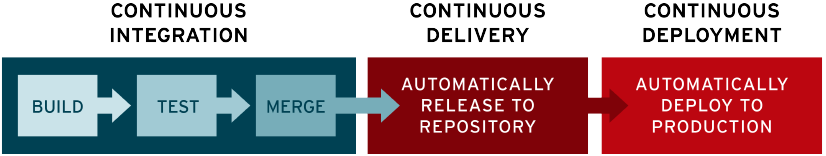
\includegraphics[width=0.85\textwidth]{ci-cd-flow-desktop}
    \caption{\textit{CI/CD} tok}
    \label{fig:cicd}
\end{figure}

Od slučaja do slučaja, na šta se termini konkretno odnose zavisi od toga koliko je automatizacije 
ugrađeno u \textit{CI/CD} tok. Mnoga preduzeća započinju automatizaciju dodavanjem kontinualne integracije, 
nakon čega uvode automatizaciju dostavljanja i raspoređivanja.

\subsubsection{Kontinualna integracija}
U razvoju modernih aplikacija, cilj je da više programera istovremeno radi na različitim delovima 
aplikacije. Međutim, ukoliko je organizacija postavljena tako da se spajanje koda sa svih grana 
vrši u jednom danu, takav posao može biti monoton, manuelan i dugotrajan. To se dešava u slučajevima 
kada programer vrši izmene na aplikaciji i na taj način povećava šansu za nastajanje konflikta sa 
izmenama koje istovremeno prave drugi programeri.

Kontinualna integracija (\textit{CI}) pomaže programerima da spoje izmene na kodu na deljenu granu češće, 
čak i na dnevnom nivou. Nakon spajanja izmenjenih delova koda, izmene se validiraju tako što se 
automatski gradi aplikacija i pokreće se više nivoa automatskog testiranja. To znači da se testira 
sve, od klasa i funkcija do različitih modula koji su deo aplikacije. Ako automatski testovi pronađu 
konflikt između novog i postojećeg koda, \textit{CI} olakšava rešavanje konflikata jer pomaže u 
pronalaženju uzroka konflikta. Uspešan \textit{CI} označava da su nove izmene koda 
na aplikaciji regularno izgrađene, testirane i pripojene deljenom repozitorijumu.

\subsubsection{Kontinualno dostavljanje}
Nakon automatskog građenja aplikacije i testiranja u \textit{CI}, kontinualno dostavljanje automatizuje 
puštanje prethodno validiranog koda u repozitorijum. Kako bismo imali efektivan proces kontinualne 
dostave, važno je da imamo već ugrađen \textit{CI} u protoku. Cilj kontinualnog dostavljanja jeste postojanje 
baze koda koja je uvek spremna za raspoređivanje na produkciono okruženje.

U kontinualnom dostavljanju, svaka faza, počevši od spajanja izmenjenog koda do dostavljanja 
verzija spremnih za produkciju, podrazumeva automatsko testiranje i automatizaciju raspoređivanja 
koda. Može se smatrati odgovorom na slabu preglednost i komunikaciju između tima 
programera i poslovnog tima. Iz tog razloga, svrha kontinualnog dostavljanja jeste da omogući 
raspoređivanje novog koda brzo, jednostavno i uz minimalne napore.

\subsubsection{Kontinualno raspoređivanje}
Poslednja faza \textit{CI/CD} toka je kontinualno raspoređivanje. Kao dodatak kontinualnom dostavljanju, 
koji automatizuje isporuku verzija spremnih za produkciju, kontinualno raspoređivanje automatizuje 
puštanje aplikacije u produkciju. U velikoj meri se oslanja na dobro osmišljeno automatsko testiranje.

U praksi, kontinualno raspoređivanje znači da izmene na aplikaciji mogu biti na produkciji za samo 
nekoliko minuta (pod pretpostavkom da su automatski testovi uspešno završeni).

Kontinualno dostavljanje i kontinualno raspoređivanje su povezani koncepti i mogu se koristiti naizmenično. 
I jedan i drugi tiču se automatizacije određenih faza u distribuiranju aplikacije, 
međutim, nekada se koriste i odvojeno u cilju prikaza količine automatizacije koja se odvija.

Sve povezane prakse \textit{CI/CD} čine raspoređivanje aplikacije manje rizičnim, stoga je lakše pustiti 
promene u aplikaciji u delovima, pre nego odjednom~\cite{CI_CD}.

\subsubsection{GitHub Akcije}
Za verzionisanje koda se može koristiti \textit{GitHub}. Pored verzionisanja, on pruža i alate za automatizaciju 
kontinualne integracije, isporuke i raspoređivanja, kroz alat koji su nazvali \textit{GitHub Akcije} 
(eng. \textit{GitHub Actions}). 
\textit{GitHub Akcije} su zasnovane na događajima, što znači da mogu da pokrenu niz komandi koje će se desiti 
posle navedenog događaja. Na primer, svaki put kada neko napravi \textit{zahtev za promenu} 
(eng. \textit{Pull Request}) u repozitorijumu, može se automatski pokrenuti komanda koja pokreće 
testove. 

\textit{GitHub Akcije} koriste fajlovi u formatu \textit{YAML} kako bi se definisale komponente toka rada. Ovi fajlovi 
se čuvaju u repozitorijumu, u folderu pod nazivom \mbox{\texttt{.github/workflows}}.

Komponente koje postoje u \textit{GitHub Akcijama} su: 

\begin{itemize}
    \item Izvršilac (eng. \textit{Runner});
    \item Tok rada (eng. \textit{Workflow});
    \item Događaj (eng. \textit{Event});
    \item Posao (eng. \textit{Job});
    \item Korak (eng. \textit{Step}) i
    \item Akcija (eng. \textit{Action}).
\end{itemize}

\begin{figure}[h]
    \centering
    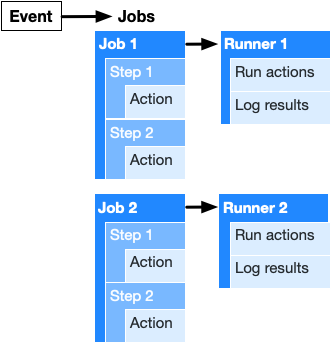
\includegraphics[width=0.5\textwidth]{overview-actions-design}
    \caption{Prikaz interakcija komponenata \textit{GitHub Akcija}}
\end{figure}

\paragraph{Izvršilac}
Izvršilac je mašina nad kojom se \textit{GitHub Akcije} izvršavaju. Izvršilac osluškuje pokrenute poslove,
pokreće jedan posao za drugim, i šalje izveštaje \textit{GitHub}-u o napretku, logovima i rezultatima. Ove 
mašine mogu da budu bazirane na \textit{Linux}, \textit{Windows} i \textit{macOS} operativnim sistemima, a svaki posao 
unutar toka rada se pokreće iz novog virtualnog okruženja~\cite{GitHubActions}.

\paragraph{Tok rada}
Tok rada je automatizovana procedura koja se definiše u repozitorijumu. Tokovi rada su sastavljeni 
od jednog ili više poslova i mogu se pokrenuti na određeni događaj ili biti zakazani u određeno vreme. 
Tok rada se može koristiti da se aplikacija izgradi, testira, spakuje, isporuči ili rasporedi na 
različita okruženja.

\paragraph{Događaji}
Događaj je specifična aktivnost koja pokreće tok rada. Na primer, aktivnost može nastati kad neko napravi 
zahtev za promenu. Aktivnost ne mora da bude u okviru \textit{GitHub}-a. Ona može da predstavlja i poziv od strane 
nekog eksternog sistema.

\paragraph{Posao}
Posao predstavlja skup koraka koji treba da se izvrše u okviru istog izvršioca. Tok rada sa više poslova 
će pokrenuti ove poslove u paraleli. Naravno, tok rada se može podesiti tako da izvršava poslove 
sekvencijalno. Na primer, tok rada može imati dva sekvencijalna posla koji izgrađuju i testiraju kod, 
gde je posao za testiranje zavisan od toga da li kod uopšte može da se izgradi. Ako posao za izgradnju 
ne uspe, posao za testiranje se neće ni pokretati.

\paragraph{Korak}
Korak predstavlja jedan zadatak koji može pokrenuti komandu unutar posla. Korak može biti ili akcija ili 
komandni skript. Svaki korak unutar posla se izvršava nad istim izvršiocem, što dozvoljava akcijama da 
dele podatke između sebe.

\paragraph{Akcija}
Akcije predstavljaju samostalne komande koje se mogu kombinovati u korake kako bi sačinile jedan posao.
Akcije su najmanje portabilne jedinice građe toka rada. Korisnici mogu sami da naprave svoje akcije
ili da koriste akcije koje su napravljene od strane \textit{GitHub} zajednice. 

